\documentclass[12pt]{article} %Basic document type
\usepackage{times} %Font 
\usepackage{amsmath} %For matrices
\usepackage{amssymb}
\usepackage[section]{placeins} %Allows FloatBarrier command
\usepackage[utf8]{inputenc} %Font encoding
\usepackage[margin=1.25in]{geometry} %Adjust margins
\usepackage{graphicx} %Allows picture import
\usepackage{pdfpages} %Including pdf files 
\usepackage{setspace}
\usepackage{fancyhdr}
\usepackage{appendix}
\graphicspath{{images/}} %Allows picture impor
\pagestyle{fancy}
\fancyhf{}
\fancyhead[L]{A Real-Time Object Tracking System}
\fancyhead[R]{ECSE 456}
\fancyfoot[C]{\thepage}
\renewcommand{\headrulewidth}{1pt}
\renewcommand{\footrulewidth}{1.5pt}
\newcommand{\HRule}[1][\medskipamount]{\par
  \vspace*{\dimexpr-\parskip-\baselineskip+#1}
  \noindent\rule{\linewidth}{0.2mm}\par
  \vspace*{\dimexpr-\parskip-.5\baselineskip+#1}}
\begin{document}
\begin{titlepage}
\begin{center}
\textsc{\huge McGill University}\\[1.5cm]
\textsc{\LARGE Department of Electrical \& Computer Engineering}\\[1.5cm]
\textsc{\Large ECSE 456 - Final Report}\\[3cm]
\HRule
{\huge \bfseries A Real-Time Object Tracking System \\[.3cm] }
\HRule 
\vspace{1.5cm}
\noindent
\begin{minipage}{0.4\textwidth}
\begin{flushleft} \large
\emph{\Large Authors:}\\
\vspace{.2cm}
Benjamin \textsc{Brown} \\
\textit{benjamin.brown2@mail.mcgill.ca} \\
260450182 \\
\vspace{.2cm}
Taylor \textsc{Dotsikas} \\
\textit{taylor.dotsikas@mail.mcgill.ca} \\
260457719
\end{flushleft}
\begin{flushleft} \large
\emph{\Large Supervisors:}\\
\vspace{.2cm}
Warren \textsc{Gross, Prof.}\\
\vspace{.2cm}
Arash \textsc{Ardakani} 
\end{flushleft}
\end{minipage}%
\end{center}
\end{titlepage}
\pagebreak
\section*{Abstract}
Video processing represents an extremely relevant challenge as both the demand for intelligent, aware systems and the quality of modern video technology increases. This increase in quality comes at a cost of large amounts of data being handled under strict time constraints \cite{3}. This project aimed to study how a common video processing algorithm such as object motion tracking can be accelerated using custom hardware. This report concludes on the background, design, and findings of Phase 1 of the project; where platform research, algorithm research, and software implementation was performed. It was clear that an FPGA would be the best solution for fast, low power hardware implementation and a Kalman filter based algorithm was the best solution for a predictive algorithm not prone to noise. Finally, the large amount of time the software needed to process relatively short videos proved that direct hardware implementation of the algorithm is essential for applications. Software implementation was performed in MATLAB, and hardware implementation will be done on an Altera Cyclone II FPGA during Phase 2 of the project.
\section*{Acknowledgments}
The authors would like to thank Professor Warren Gross, for undertaking the responsibility of supervising this project. We would also like to thank Arash Ardakani for all of his advice, help, and time spent meeting with us throughout the semester. Finally, we would like to thank anyone who contributed to the wealth of online resources about object tracking that we hope to contribute to.
\pagebreak
\tableofcontents
\pagebreak
\section{Abbreviations \& Notation}
\begin{itemize}
\item[] FPGA - Field Programmable Gate Array
\item[] ASIC - Application Specific Integrated Circuit
\item[] CPU - Central Processing Unit
\item[] DFG - Delta Frame Generation
\end{itemize}
\section{Introduction}
\subsection{Motivation}
Scene recreation and analysis is imperative in digital systems that must understand and react to events in their environment. Some typical examples of this include surveillance, robotics, and human-computer interaction. A variety of sensors can be employed for such a task including ultrasonic, radar, and passive infrared, but all of these sensors do not come close to modeling an environment as completely as a video camera. With the increase in image quality and device accessibility, the video camera seems like the obvious solution. \\\\
However, due to the vast amount of data and system imposed processing time constraints, video processing is a challenge. For instance, the transition to a high-definition video platform produces six times more data than the previous standard-definition one \cite{3}. This project aims to study how a complex video processing algorithm such as real-time object tracking can be greatly accelerated when implemented directly in hardware. Object tracking represents an excellent example of the preceding challenges because it requires capturing an image of a scene, processing the image to locate the object in motion, and reconstructing said scene with emphasis placed on the motion, all in real-time.
\subsection{Applications}
The device generates object localization data that can be used by other systems. Systems that require responsive and accurate data for real time use can are the main applications. These secondary systems can now react to moving objects in the selected environment. \\\\
Specifically our algorithm tracks a single object from a camera that watches a stationary environment. This makes our design ideal for tracking a disturbance in the field of view. For example, the addition of our device to a camera surveillance system would provide data about where and when disturbances take place. This information could be used to quickly react to disturbances such as a trespassers on private property.\\\\
Dedicated hardware allows for simpler connectivity to secondary systems. It presents a modular design which is ideal for testing purposes and debugging. If object tracking needs to be performed on higher definition video, dedicated hardware has its own memory which can be specifically allocated for handling larger image frames. Performance depends on the technical specifications of the hardware being used. Our current hardware is limited due to our budget, however it would be possible to upgrade the hardware to match the needs of the desired application. \\\\
The kalman filter in our design tracks the object more smoothly and can also guess the location of the object if it disappears from the view temporarily. This further enhances the performance of secondary systems by providing them with more accurate and useful object tracking data, which is the main goal of the device.
\section{Background}
\subsection{Video Processing}
The most fundamental way of understanding video data is to consider it as a collection (static) or stream (real-time) of discrete images called frames. A frame is an $MxN$ matrix of pixels. Each pixel is the smallest, discrete element of the image, and store intensity data about the image. There are many different ways of representing intensity in a pixel. In the case of a color image, the pixel contains multiple values that describe the color space. Common representations of the color space are RGB or YCbCr \cite{1}. In both of these models, each pixel has 3 values.  Since MATLAB's \texttt{VideoReader} class uses RGB, for convenience, this color space is used for the remainder of the project. A single color RGB frame is mathematically described as an $MxNx3$ matrix with the form
\begin{equation}
F_i = 
\begin{bmatrix}
(R_{11}, G_{11}, B_{11}) & ... & (R_{1N}, G_{1N}, B_{1N}) \\
 & &\\
... & ... & ... \\
 & &\\
(R_{M1}, G_{M1}, B_{M1}) & ... & (R_{MN}, G_{MN}, B_{MN}) 
\end{bmatrix}
.
\end{equation}
Where
\[
i = 1, 2, ... , n.
\]
\[
0 \leq R_{ij}, G_{i,j}, B_{i,j} \leq 256
\]
The first frame, $F_1$, is defined as the \textit{base frame}, and the remaining frames are defined as the \textit{current frame} for processing. If a video is $t$ seconds long, the \textit{frame rate }is defined as
\begin{equation}
f = \frac{t}{n}.
\label{eq:framerate}
\end{equation}
In the case of a black and white image, the pixel contains a single value that represents the grayscale intensity. Similar to $F_i$, the grayscale frame also contains $n$ frames, and its elements, $Y_{ij}$, are limited between 0 and 256. However, it is an $MXN$ matrix only. It will become apparent later that conversion between RGB and grayscale is imperative for many video processing algorithms. Unsurprisingly, there are multiple ways to do this. The colorimetric conversion principle converts RGB to grayscale using the following weighted sum:
\begin{equation}
Y_{ij} = .2126 \cdot R_{ij} + .7152 \cdot G_{i,j} + .0722 \cdot B_{i,j}.
\end{equation}
Finally it should be mentioned that video data can be streamed in either progressive or interlaced format. Progressive format is the standard one frame at a time while interlaced divides the frames in half into fields. Each field contains either odd or even rows of it's corresponding frame. While this does requiring processing more frames, it gives a clearer, smoother picture as there are less scene changes between frames \cite{1}. This design choice plays a larger role in Phase 2 of the project, since software implementation uses static (pre-recorded) videos.
\subsection{Optical Flow}
Optical flow addresses the idea of determining apparent motion based on changes in image intensity (i.e. brightness) over space and time \cite{4}. All of the proposed differential and matching (feature-based) techniques proposed in Trucco \& Verri \cite{4} go beyond the scope of this project. The simplest of these algorithms involve derivatives of the brightness constancy equation and a least squares solution at each pixel. Not only would they be difficult to implement in both software and hardware, but they produce what is known as the motion field of the image. This is more information than what is needed for the Kalman filter algorithm that is discussed next, which requires simply knowing the $(x,y)$ coordinate of the object in each frame. \\\\
A far simpler, less robust approach is used of locating the object in motion for each frame known as Delta Frame Generation (DFG) \cite{8}. This method makes the following assumptions about the image:
\begin{enumerate}
\item The object of interest is in motion.
\item The object of interest is the only part of the scene in motion.
\item The first frame of the sequence does not contain the object.
\item The lighting and background of the scene does not change between frames.
\end{enumerate}
The delta frame is then calculated as 
\begin{equation}
\Delta_i = | F_i - F_1 |.
\end{equation}
Where $F_i$ is the current grayscale frame and $F_1$ is the base grayscale frame discussed in the previous section. Assuming the above assumptions hold, the delta frame, $\Delta$, will be non-zero for only the object. Knowing that $\Delta$ contains only the object, drawing a line from the top/bottom most points, and finding its intersection with another line from left/right most points produces the center point of the object. The mathematical background for this is as follows. By means of simple search algorithms, the top, bottom, left, and right most points are located as
\[
p_t = (x_1, y_1) ,
\]
\[
p_b = (x_2, y_2) ,
\]
\[
p_l = (x_3, y_3) ,
\]
\[
p_r = (x_4, y_4) .
\]
Then the two lines are given as 
\[
l_1(t,b):
\]
\[
l_2(l,r):
\]
\subsection{Kalman Filter}
A Kalman filter is used to combine continuous predictions from a theoretical system model with continuous measurements from a real implementation of the same system. This is done to help reduce the effects of noise on system measurements, and can provide a prediction of the system's next state if for some reason the measurements fail or contain lots of noise. Implementation of a Kalman filter is highly intuitive for a sensor that has been characterized with testing. But for object tracking, it is much more difficult to understand as all of the Kalman filter jargon is focused around "sensors" and "measurements" that sound odd when referring to an object tracking system. \\\\
The Kalman filter equations can be divided into two key sets: the predication equations and the update equations \cite{4}, \cite{12}.\\\\
\textbf{Prediction Equations:}
\begin{equation}
\vec{x_{k+1}} = F \cdot \vec{x_k} + B \cdot \vec{u_k}
\label{eq:firstkalman}
\end{equation}
\begin{equation}
P_{k+1} = F \cdot P_k \cdot F^T + Q
\end{equation}
\textbf{Intermediate Calculations:}
\begin{equation}
\vec{y_{k+1}} = \vec{z_k} - H \cdot \vec{x_{k+1}}
\end{equation}
\begin{equation}
S_{k+1} = H \cdot P_{k+1} \cdot H^T + R
\end{equation}
\begin{equation}
K_{k+1} = P_{k+1} \cdot H^T \cdot S_{k+1}^{-1}
\end{equation}
\textbf{Update Equations:}
\begin{equation}
\hat{\vec{x_{k+1}}} = \vec{x_{k+1}} + K_{k+1} \cdot \vec{y_{k+1}}
\end{equation}
\begin{equation}
\hat{P_{k+1}} = (I - K_{k+1} \cdot H) \cdot P_{k+1}
\end{equation}
There are a few key observations that can be immediately made about this set of equations. Note that the distinction between intermediate calculations and predication equations is one that is not usually made in descriptions of Kalman filtering like the one by Trucco \& Verri [4]. However, from an implementation perspective this distinction makes sense, as the system in which the Kalman filter is placed in (or main algorithm) is blind to these equations. Also notice that matrices and vectors without subscripts are ones that do not change each iteration, and remain constant from initialization to completion. \\\\
While all elements in this set of equation have physical meanings and distinct characteristics, for the sake of simplicity the only once that need to be discussed in detail are the inputs, outputs, and constant variables. The two quantities already discussed are the measurement vector $\vec{z}$ of length $m$ and the state vector $\vec{x}$ of length $n$. For this application, $m = 2$ since by methods of optical flow discussed previously we are able to get a 2D Cartesian coordinate for the object.
\begin{equation}
\vec{z} = \begin{bmatrix}
x \\
y \\
\end{bmatrix}
\end{equation}
The length of the state vector depends on the model that has been chosen for the system. Two common models for object tracking applications are the constant velocity model and the constant acceleration model. The assumptions made in these models is self explanatory; $n=4$ for constant velocity and $n=6$ for constant acceleration. In this system, the constant velocity model is used.
\begin{equation}
 \vec{x} = \begin{bmatrix}
x_p \\
y_p \\
v_x \\
v_y
\end{bmatrix}
\end{equation}
The next system dependent variable is the state transition matrix $F$ which is $nxn$. As equation ~\ref{eq:firstkalman} indicates, it describes how the theoretical, predicted behavior of the system changes with each iteration \cite{12}. For a 2D constant velocity model, this matrix is just implementing kinematic equations:
\begin{equation}
x_{new} = x_{old} + t * v_x
\end{equation}
With a similar equation existing for $y$. In matrix form this is 
\begin{equation}
F= \begin{bmatrix}
1 & 0 & f & 0 \\
0 & 1 & 0 & f \\
0 & 0 & 1 & 0 \\
0 & 0 & 0 & 1
\end{bmatrix}.
\end{equation}
Where $f$ is the frame rate (i.e. the time step) described in equation ~\ref{eq:framerate}. Also stemming from equation ~\ref{eq:firstkalman}, the vector $\vec{u}$ describes any external inputs applied to the system between iterations. For a simple, constant velocity object tracking system, there are none. This makes the vector irrelevant as well the associated matrix $B$. Getting back to the measurements, the only constant matrix that incorporates $m$ is the measurement model $H$ \cite{4}. This is an $mxn$ matrix that relates the predicated state to the measured value. For this application, it should take the vector $x$ of length 4 and place it in the same vector space as $z$ of length 2. Thus,
\begin{equation}
H = \begin{bmatrix}
1 & 0 & 0 & 0 \\
0 & 1 & 0 & 0 
\end{bmatrix}.
\end{equation}
The final two constant matrices that must be initialized prior to starting are $Q$ ($nxn$) and $R$ ($mxm$). These matrices are related to the error in the theoretical model (i.e. air resistance, friction) and the error in the measurement model (i.e. your "sensors", in this case optical flow) respectively \cite{12}. In theory, if there are vectors $\vec{w}$ and $\vec{v}$ that characterize the error in the model and measurement respectively, then $Q$ and $R$ should be diagonal matrices containing the variance of these vectors \cite{4}. \\\\
The final, and perhaps most important, value that should be touched on is the co-variance matrix $P$ ($nxn$) which changes with each iteration. In simple terms, this matrix is a measure of how well the measurements follow the model, and thus how accurate the filter is \cite{12}. Unlike the previously discussed values, $P$ will eventually converge to certain values do to the iterative nature of the algorithm.
\subsection{Fixed vs. Floating-Point}
Ben
\section{Requirements}
Several requirements had to be met so that the device could be viable for use. We placed a strong emphasis on code efficiency in our software development. Computational time dedicated to video processing needs to be kept at a minimum so that the object tracking is done as close to real time as possible. The main goal is to have a live video feed from a camera displayed on a screen and a cursor tracking the object. This will be visual proof that the device works. If our code was inefficient or too intensive, there would be a delay between what was actually happening in front of the camera, and the output video feed that has the object located. The device would not have much use if there was a lot of lag. There will be some delay as it would be impossible to accomplish the necessary computations instantly, but it is possible to minimize the delay so that it is barely noticeable. This is why it was crucial to make sure computations are not redone if they don't need to be and unnecessary computations are removed. Every computation needs to be done in the optimal way considering we don't have accesses to more advanced hardware. These optimization challenges will be more apparent when we begin hardware implementation with VHDL. The hardware limitations of the FPGA certainly pose some constraints to our design but we should be able to obtain a good result with it. \\\\
All other algorithm based requirements have been met at this point in development. The ability to filter out noise and locate a single object has been implemented in our Matlab code. 


\section{Design}
\subsection{Platform}
In this section we look to formally justify the aforementioned choice of an FPGA, and specifically an Altera FPGA, for hardware implementation in comparison to other embedded hardware choices. 
\subsection{Algorithm}
Discuss the merits of the algorithms we researched and why we chose DFG with a Kalman filter.
\subsection{Software}
Discuss how the software works.
\begin{figure}[h]
\centering
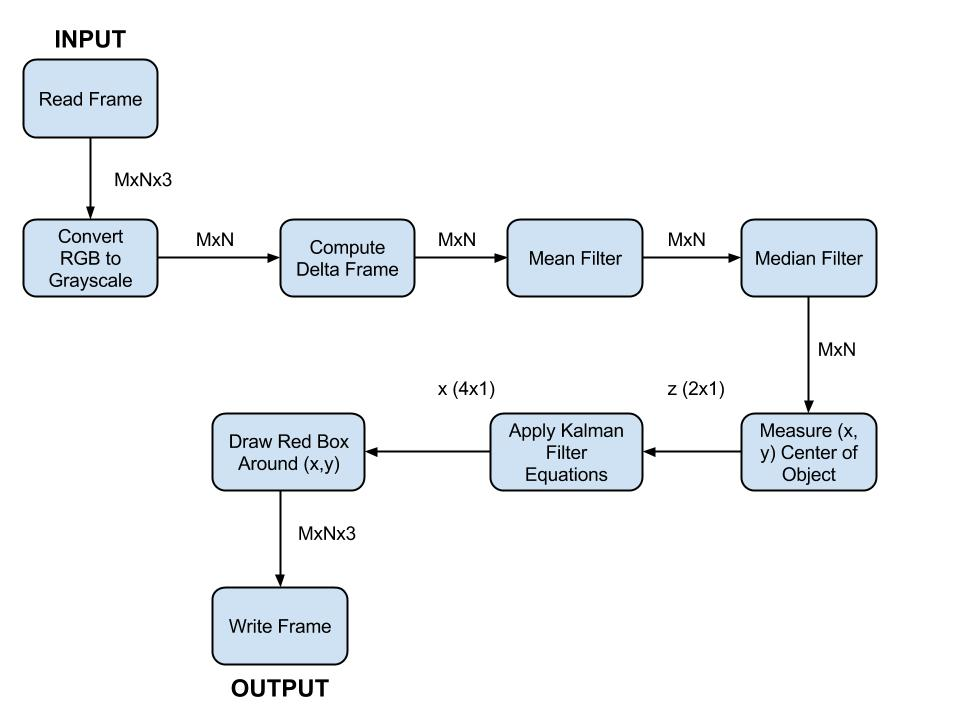
\includegraphics[width=0.75\textwidth]{./images/software_flow.jpg}
\caption{Software Flowchart}
\label{fig:sw_flow}    
\end{figure}
\section{Future Work}
Ben \& Taylor
\section{Impact on Society}
Taylor
\section{Allocation of Work}
Ben \& Taylor
\section{Conclusion}
Ben \& Taylor
\newpage
\begin{thebibliography}{11}
\bibitem{1}
F. Roth, “Using low cost FPGAs for realtime video processing”, M.S. thesis, Faculty of Informatics, Masaryk University, 2011.
\bibitem{2}
A. Saeed et al., “FPGA based Real-time Target Tracking on a Mobile Platform,” in 2010 International Conference on Computational Intelligence and Communication Networks, 2010, pp. 560-564.
\bibitem{3}
”Video and Image Processing Design Using FPGAs.” Altera. 2007. January 2014. 
http://www.altera.com/literature/wp/wp-video0306.pdf  
\bibitem{4}
E. Trucco and A. Verri, “Chapter 8 - Motion,” in Introductory Techniques for 3D Computer, pp. 177- 219.
\bibitem{5}
S.A. El-Azim et al., “An Efficient Object Tracking Technique Using Block-Matching Algorithm”, in Nineteenth National Radio Science Conference, Alexandria, 2002, pp. 427 - 433.
\bibitem{6} 
Caner et al., “An Adaptive Filtering Framework For Image Registration”, IEEE Trans. Acoustics, Speech, and Signal Processing, vol. 2, no. 2, 885-888. March, 2005. 
\bibitem{7}
Yin et al. \textit{Performance Evaluation of Object Tracking Algorithm} [Online]. Available: http://dircweb.kingston.ac.uk/ 
\bibitem{8}
G. Shrikanth, K. Subramanian, “Implementation of FPGA-Based object tracking algorithm,” Electronics and Communication Engineering Sri Venkateswara College of Engineering, 2008.
\bibitem{9}
E. Pizzini, D. Thomas, “FPGA Based Kalman Filter,” Worcester Polytechnic Institute, 2012.
\bibitem{10}
M. Shabany. (2011, December 27). \textit{Floating-point to Fixed-point Conversion} [Online]. Available: http://ee.sharif.edu/~digitalvlsi/Docs/Fixed-Point.pdf
\bibitem{11} 
N. Devillard. (1998, July). \textit{Fast median search: an ANSI C implementation} [Online]. Available: http://ndevilla.free.fr/median/median.pdf
\bibitem{12}
D. Kohanbash. (2014, January 30). \textit{Kalman Filtering - A Practical Implementation Guide (with code!)} [Online]. Available: http://robotsforroboticists.com/kalman-filtering/
\end{thebibliography}
\newpage
\appendix
\appendixpage
\section{Additional Figures} \label{sec:add}
\end{document}